\documentclass[tikz,border=3pt]{standalone}
\usepackage{newtxtext,newtxmath}
\newcommand{\avgsim}{\operatorname{avgSim}}
\usetikzlibrary{arrows.meta,positioning}
\definecolor{paperblue}{HTML}{2F6DB0}
\definecolor{paperred}{HTML}{C83E4D}
\definecolor{papergold}{HTML}{E3A008}
\definecolor{papergreen}{HTML}{2E8B57}
\definecolor{paperneutral}{HTML}{F1F3F5}
\begin{document}
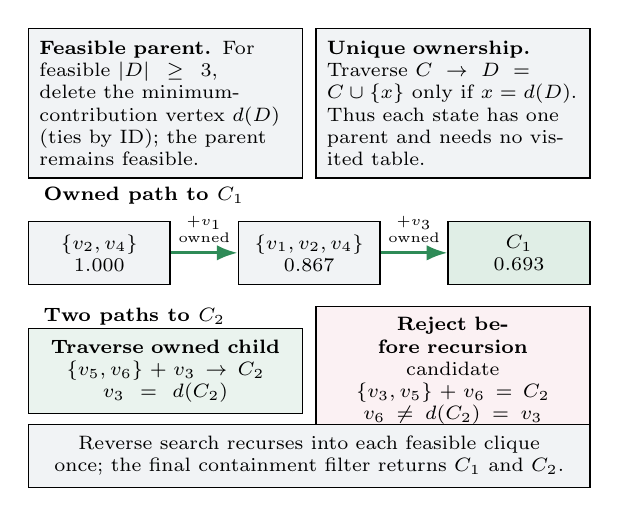
\begin{tikzpicture}[
  font=\scriptsize,
  >=Latex,
  rule/.style={draw=black, line width=0.55pt,
    minimum height=19mm, text width=32mm, align=left, inner sep=1.4mm},
  state/.style={draw=black, line width=0.55pt,
    minimum height=8mm, text width=16mm, align=center, fill=white,
    inner sep=1.0mm},
  route/.style={draw=black, line width=0.55pt,
    minimum height=10mm, text width=32mm, align=center, inner sep=1.4mm},
  accepted/.style={->, draw=papergreen, line width=1.0pt},
  phase/.style={font=\scriptsize\bfseries, anchor=west}
]
\node[rule, fill=paperneutral] (parent) at (0,0)
  {\textbf{Feasible parent.} For feasible $|D|\geq3$, delete the
   minimum-contribution vertex $d(D)$ (ties by ID); the parent remains feasible.};
\node[rule, fill=paperneutral] (owner) at (3.65,0)
  {\textbf{Unique ownership.} Traverse $C\rightarrow D=C\cup\{x\}$ only
   if $x=d(D)$. Thus each state has one parent and needs no visited table.};

\node[phase] at (-1.67,-1.18) {Owned path to $C_1$};
\node[state, fill=paperneutral] (e24) at (-0.84,-1.90)
  {$\{v_2,v_4\}$\\$1.000$};
\node[state, fill=paperneutral] (t124) at (1.825,-1.90)
  {$\{v_1,v_2,v_4\}$\\$0.867$};
\node[state, fill=papergreen!15] (c1) at (4.49,-1.90)
  {$C_1$\\$0.693$};
\draw[accepted] (e24) -- node[above,font=\tiny,align=center] {$+v_1$\\owned} (t124);
\draw[accepted] (t124) -- node[above,font=\tiny,align=center] {$+v_3$\\owned} (c1);

\node[phase] at (-1.67,-2.71) {Two paths to $C_2$};
\node[route, fill=papergreen!10] (keep) at (0,-3.40)
  {\textbf{Traverse owned child}\\
   $\{v_5,v_6\}+v_3\rightarrow C_2$\\
   $v_3=d(C_2)$};
\node[route, fill=paperred!7] (drop) at (3.65,-3.40)
  {\textbf{Reject before recursion}\\
   candidate $\{v_3,v_5\}+v_6=C_2$\\
   $v_6\neq d(C_2)=v_3$};

\node[route, fill=paperneutral, text width=68.5mm, minimum height=8mm]
  (result) at (1.825,-4.48)
  {Reverse search recurses into each feasible clique once; the final containment
   filter returns $C_1$ and $C_2$.};
\end{tikzpicture}
\end{document}
